\section{Journées zen}

Date: 11/02/2008

\begin{multicols}{2}

Après Jaipur, 2h30 de bus et nous voila à Ajmer, petite ville de 250.000 habitants si nos souvenirs sont bons. Le principal avantage du lieu est de se situer sur de nombreuses lignes de bus et d'être à seulement 15 km de Pushkar, ville de pàlerinage, très réputée pour sa beauté. Nous n'y avons donc passé qu'une nuit et qu'une journée. Toutefois nous en avons profité au maximum pour nous balader, prendre le soleil et admirer le paysage. Tout d'abord, visite du Temple Rouge Jaïn, qui nous a révélé une magnifique maquette de ville aux bateaux flottants dans les cieux, le tout recouvert de 500kg de feuillles d'or. Les murs étaient même sculptés en colonnes brillantes de vert, de rouge, de bleu.

Nous avons continué notre route jusqu'à un fort non loin. Il s'agit d'un musée contenant des tablettes de pierres gravées d'écritures et de scupltures à l'effigie des dieux. La cour interieure était tellement verdoyante et paisible que nous y avons déposé nos sacs pour une halte détente, farniente et bouquinage. L'Inde, lorsqu'elle est calme, est propice au repos et à la reflexion. Le lac fut notre dernière visite dans cette ville. Le parc est accueillant et vivant, les quais sont en marbre avec des autels et l'eau calme reflète les montagnes environnantes. Premier changement radical de décor pour nous, ca ressemble plus au desert.

Le soir pour venir à Pushkar nous avons comme à notre habitude pris le bus. Enchantés dès l'arrivée par la petite bourgade de 15.000 habitants (ou plutôt ce qu'on arrive à en voir entre la station de bus et le premier hôtel où l'on entre), nous avons pu profiter de la suite du spectacle lors d'une balade dans le bazar, encore baigné de soleil. De retour le soir, on constate avec ravissement que notre hôtel porte bien son nom de Lake View. La terrasse (qui est le toit, je pense que vous l'aurez compris, comme partout en Inde) offre une vue imprenable sur le lac sacré de Pushkar, où viennent se baigner de nombreux fidèles. A cette heure, le soleil se couche, libérant des lueurs jaunes, oranges et violettes dans le ciel, l'eau est tranquille, les montagnes presque bleues et les lumières de la ville commencent à s'allumer. Nous restons là un long moment à admirer le soleil qui descend puis s'éteint. Le soir, repas autour du feu en compagnie d'un Français et des Indiens du restaurant sur fond de Bob Marley. Ce fut une journée tout à notre rythme, tres agréable.

Aujourd'hui aussi, du coup, nous en avons profité juste en marchant, en faisant quelques emplettes et en profitant de la terrasse de l'hôtel. J'ai eu la chance, mais aussi l'audace de rentrer dans un temple, d'offrir des fleurs à Krishna et de lui faire une offrande de fleurs dans l'eau du lac. C'est une expérience qui je crois m'a beaucoup marquée, surtout moi qui suis si émotive, j'ai été tres touchée.  Maintenant que la nuit est tombée, nous avons profité de cette ambiance si différente pour faire un saut jusqu'ici vous donner des nouvelles et vous montrer quelques photos.

\hspace*{-0.65cm}
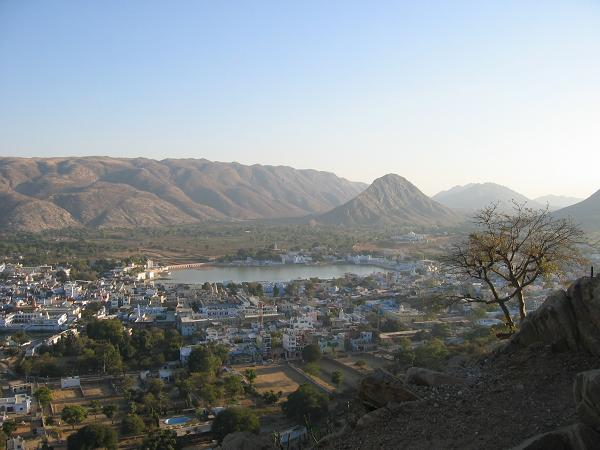
\includegraphics[width=4.8cm]{articles/Journees-zen/pushkar.jpg}
La ville de Pushkar

\end{multicols}
